% Asset ID: AS2ForcesTikZ-010
% Source: Chapter 5/7 Forces Transcript + MechYr2 Chapter 7 Applications of Forces PDF
% Related lesson section: Core Theory: Strings, pulleys and connected particles
% Purpose: Show connected particles over a smooth pulley with common tension T.
\documentclass[tikz,border=8pt]{standalone}
\usepackage{amsmath}
\usetikzlibrary{arrows.meta, angles, quotes, decorations.pathmorphing}
\begin{document}
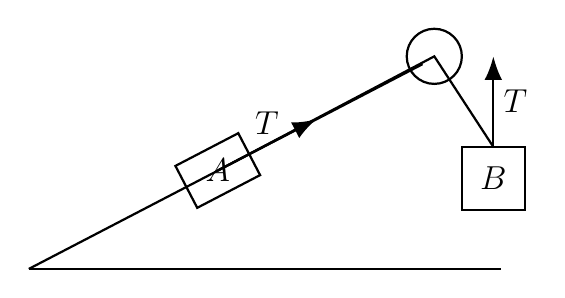
\begin{tikzpicture}[force/.style={-{Latex[length=3mm]}, thick}, comp/.style={-{Latex[length=3mm]}, thick, dashed}, label/.style={font=\large}, note/.style={font=\normalsize}]

\coordinate (A) at (0,0); \coordinate (B) at (6,0); \coordinate (C) at (5,2.6); \draw[thick] (A)--(B); \draw[thick] (A)--(C); \coordinate (P) at (5.15,2.7); \draw[thick] (P) circle (0.35);
\coordinate (PA) at (2.4,1.25); \begin{scope}[shift={(PA)}, rotate=27.5]\draw[thick] (-0.45,-0.3) rectangle (0.45,0.3); \node[label] at (0,0) {$A$};\end{scope}
\draw[thick] (5.5,0.75) rectangle ++(0.8,0.8); \node[label] at (5.9,1.15) {$B$}; \draw[thick] (PA)--(P)--(5.9,1.55); \draw[force] (PA)--++(1.25,0.65) node[midway,above,label] {$T$}; \draw[force] (5.9,1.55)--++(0,1.15) node[midway,right,label] {$T$};
\end{tikzpicture}
\end{document}
